\chapter{Geometrische Beziehungen zwischen Punktekorrespondenzen}
\label{sec:HFE}

Das Ziel dieser Masterarbeit ist es Punkte im dreidimensionalen Raum aus einer Stereoskopischen Aufnahme zweier Kameras zu rekonstruieren. Bis jetzt wurde die Bildaufnahme einer einzigen Kamera betrachtet. Jedoch kann eine Kamera allein nicht räumlich sehen. Um Räumlichkeit aus Bilder zu rekonstruieren, müssen mindestens zwei Aufnahmen der gleichen Szene aus unterschiedlichen Blickwinkeln aufgenommen werden. Innerhalb dieser Aufnahmen müssen Punktekorrespondenzen gesucht werden. Korrespondierende Punkte zeichnen sich dadurch aus, dass sie die Abbildungen ein und des selben projektiven Punkts im Raum sind. Für diese Punkte muss dann eine gemeinsame Abbildungsvorschrift aufgestellt werden. Über die Abbildungsvorschrift können dann Schlüsse auf die Kameraparameter der beiden Kameras gezogen werden. Im ersten Schritt wird eine Abbildungsvorschrift für die Korrespondenzanalyse von Punkten auf einer Ebene aufgestellt. Im zweiten Schritt wird diese Abbildungsvorschrift für die Lautkorrespondenz zwischen willkürlichen Punkten im Raum entwprechend erweitert. \\


Im letzten Schritt wird die berechnung des ersten Falls dargelegt, die berechnung des zweiten falls folgt im zuge der Szenenrekonstruktion im Virtuellen Beispiel.


Zum detektieren solcher Punktekorrespondenzen gibt bereits Algorihtmen, wie Beispielsweise den SURF-Algorithmus\cite{SURF}, welcher auch in dieser Arbeit verwendet wurde.  

 
 \section{Korrespondenzanalyse für Punkte auf einer Ebene (Homographie)}
 
 Es wird der direkte Zusammenhang zwischen zwei Bildpunkten auf unterschiedlichen Kamerabildebenen aus ein un demselben Punkt hergeleitet. 

%Solche Bildpunkte auf unterschiedlichen Bildebenen werden korrespondierende Punkte genannt.
 
  In diesem Abschnitt wird davon ausgegangen dass die z-Komponente des Ursprungpunktes $M_{\delta z}$ bekannt ist. Dies wird in Abbildung XX schematisch dargestellt.
 
 %In diesem Abschnitt wird davon ausgegangen, dass dass der Ursprungspunkt $M_\delta=(M_{\delta x},M_{\delta y},M_{\delta z},O) $ auf einer Ebene $\pi$ mit bekannter Gleichung (muss ich das ausführen?), wie in Abbildung () dargestellt.
 
 %In diesem Abschnitt wird davon ausgegangen, dass der Ursprungspunkt $M_\delta=(M_{\delta x},M_{\delta y},M_{\delta z},O) $ eindeutig bestimmt ist, ... Bildeben 
 % auf einer Ebene liegen und damit durch M_{\delta x} und M_{\delta y}  M_{\delta z} eindeutig bestimmt werden kann. 
 
 %Ein Punkt auf der normierten Bildebene m_{n,\tau}=(m_{n,\tau x},m_{n,\tau y},1, I) 
 
 
 \begin{minipage}{\linewidth}
 	\centering
 	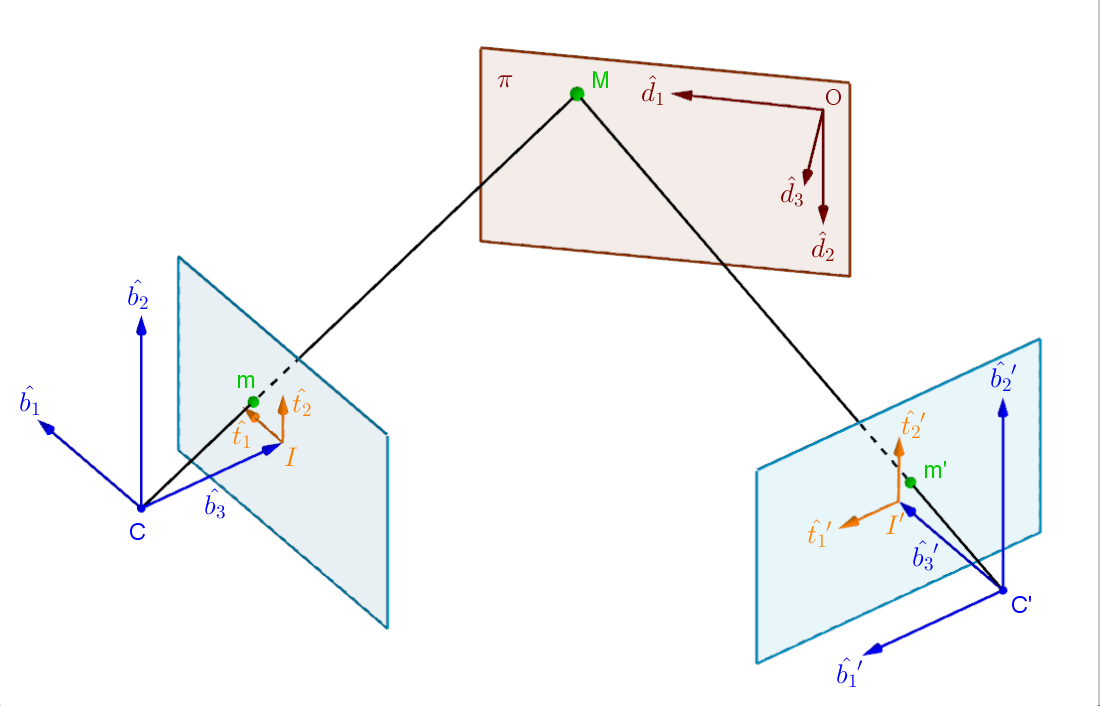
\includegraphics[width=0.8\linewidth]{images/HomographieDP_beschriftet.png}
 	\captionof{figure}{Veranschaulichung der Homographie bei zwei verschieden translatierten und rotierten Kameras.}  
 \end{minipage}\\
 
 %Ein Punkt auf der normierten Bildebene m_{n,\tau}=(m_{n,\tau x},m_{n,\tau y},1, I) lässt sich somit eindeutig zurücktransformieren indem die Gerade $\g=vec(C)+t\vec(Cm)
 
 Ein Punkt auf der normierten Bildebene $m_{n,\tau}=(m_{n,\tau x},m_{n,\tau y},1, I)$ lässt sich somit eindeutig auf die Bildebene erweitern mit 
 
 \begin{gather}
 	m_{\tau}=(m_{\tau x},m_{\tau y},m_{\tau z}, I) = M_{\delta z}(m_{n,\tau x},m_{n,\tau y},1, I)=M_{\delta z}m_{n,\tau}
 \end{gather}\\
 
 Für 2 korrespondierende Punkte $m_{\tau}$ und $m'_{\tau}$ auf 2 unterschiedlichen Bildebenen gilt der folgende Zusammenhang
 
 
 \begin{gather}
 	m_{\tau}=M_{\delta z}m_{n,\tau} = M_{\delta} \cdot P \\
 	m'_{\tau}=M_{\delta z}m'_{n,\tau} = M_{\delta} \cdot P'
 \end{gather}\\
 
 Die Projektionsmatirx $P$ beschriebt in diesem Fall nur die Abbildung auf die Bildebene und wird durch $P=K_0R$ mit der Kameramatrix $K_0$ und der Transformationsmatrix $R$ aus Kapitel 2 zusammen. Durch das Anwenden der inversen von $P$ und $P'$ von rechts auf die gleichung, werden diese zu
 
 
 \begin{gather}
 	m_{\tau}\cdot P^{-1}=M_{\delta z}m_{n,\tau}P^{-1} = M_{\delta} \\
 	m'_{\tau}P'^{-1}=M_{\delta z}m'_{n,\tau}P'^{-1} = M_{\delta}.
 \end{gather}\\
 
 Auf der rechten Seite der Gleichung steht schlieslich derselbe Ursprungspunkt, sodass wir beide gleichung zusammenfassen können. 
 
 \begin{gather}
 	m_{\tau}\cdot P^{-1} = m'_{\tau}P'^{-1} \\
 	m_{n,\tau}P^{-1}=m'_{n,\tau}P'^{-1}
 \end{gather}\\
 
 Multiplizieren wir nun P von rechts auf die Gleichung erhalten wir 
 \begin{gather}
 	m_{n,\tau}=m'_{n,\tau}P'^{-1}P=m'_{n,\tau}H
 \end{gather}\\
 
die sogenannte Homographiematirx $H=P'^{-1}P$. Diese Matrix beschreibt die direkte, eindeutige Abbildung von einem Bildpunkt auf der 2 dimensionalen Bildebene I' auf den Bildpunkt auf der Bildebene I. Mittels der inversen $Hi$ kann diese Abbildung auch rückwerts gemacht werden. 
 \\
 Mann könnte das gleichungssystem hier ausformulieren um auf die bestimmung der Kameraparameter einzugehn, wenn du willst (denke das hilft hier zwar nicht aber schaden tut warhscheinlich auch nicht so sehr)
 
 
 
 \section{Korrespondenzanalyse für willkürliche Punkte ?im Raum? (Epipolare Geometrie)}
 
 In diesem Kapitel wird der Fall einer Korrespondenzanalyse für Punkte behandelt, bei denen die z-Komponente des abzubildenden Punktes $M_{\delta z}$ nicht bekannt ist. Die Punkte können somit überall im Raum liegen und wir definieren $M_{\delta z}=k$, mit einer freien Variablen k. Für die Transformation eines Punktes im normalisiertn Bildkoordinatensystem in die nicht normalisierten Bildkoordinaten gilt somit:
 
 \begin{gather}
 	m_{\tau}=(m_{\tau x},m_{\tau y},m_{\tau z}, I) = k(m_{n,\tau x},m_{n,\tau y},1, I)=M_{\delta z}m_{n,\tau}
 \end{gather}\\
 (im nicht normalisierten Koordinatensystem befinde sich nun der Punkt auf der durch C und m(Tau) gehenden geraden, durch die Art wie die normierung funktioniert befindet sich der Objektpunkt auf geraden durch )
 
 
 
 Für 2 korrespondierende Punkte $m_{\tau}$ und $m'_{\tau}$ auf 2 unterschiedlichen Bildebenen kann folgende gleichung hergeleitet werden
 
 
 \begin{gather}
 	m_{\tau}=km_{n,\tau} = M_{\delta} \cdot P \\
 	m'_{\tau}=k'm'_{n,\tau} = M_{\delta} \cdot P'
 \end{gather}\\
 
 Wie in Kapitel 3.1 lässt sich folgende Beziehung herleiten
 
 \begin{gather}
 	km_{n,\tau}P^{-1}  = k'm'_{n,\tau}P'^{-1}.
 \end{gather}\\
 (diese gleichung repräsentiert die such nach dem Schnittpunkt der beiden Geraden wie oben gemeint)\
 
 Dies Gleichung können wir mit der Homographimatrix $H$ wiederum in 
 
 \begin{gather}
 	m_{n,\tau} =\lambda  m'_{n,\tau}H
 \end{gather}\\
 
 mit $\lambda=k/k'$. $\lambda$ beschreibt somit den relativen Unterschied der oben definierten $M_{\delta z}$. Wenn  
 
 $(\lambda m'H  =entspricht der epipollinie l)$


\textcolor{red}{(WICHTIG: dann noch zeigen was es mit den normierten Bildpunkten auf sich hat!!! sobald die rechnung wieder da ist)}


\section{geometrische Erläuterung der Epipolargeometrie}
\label{sec:epipolar} 


Auf Abbildung \ref{fig:Epipolargeometry} wird die oben beschriebene mathematische Herleitung der Epipolargeomety grafisch dargestellt.  \textcolor{red}{(Kurz darlegen was ist was in der Grafik in bezug zu den Formeln)}\\

Ein Objektpunkt $M_\delta$ wird auf die Bildebenen $I$ und $I'$ der beiden Kameras $C$ und $C'$ projiziert. Es entstehen die zueinander korrespondierenden Bildpunkte $m_\tau$ und $m'_{\tau'}$. Die durch die Bildpunkte $m_\tau$ und $m'_{\tau}$ und den entsprechenden Epipolen $e$ und $e'$ verlaufenden Epipolarlinien, sind zueinander korrespondierende Epipolarlinien. Die zum Punkt $m_\tau$ korrespondierende Epipolarlinie $l'$ beinhaltet alle zu $m_\tau$ möglichen korrespondierenden Punkte, darunter eben auch der eindeutig korrespondierende Punkt $m'_{\tau'}$.\\

 Die Epipolargeometrie beschreibt weiterhin eine Beziehung zwischen einem Bildpunkt $m$ und dessen korrespondierender Epipolarlinie $l'$. \textcolor{red}{Hier kann eine Verbindung zu den willkürlichen Tiefen hergestellt werden und anhand des Bildes gezeigt werden und anhand von Abbildung \ref{fig:Epipolarconstraint}} \\
 
Diese Beziehung ist der sogenannte ist der sogenannte \textit{Epipolar-Constraint}\cite{HZ,Zhang2014,ZZGXr}.  \textcolor{red}{(beschreibt der nicht quasi das selbe wie die Abbildungsvorschrift, also bzw hier könnte man die grafik in bezug zur gleichung bringen)}
Der \textit{Epipolar-Constraint} sagt aus, dass wenn ein 3D-Bildpunkt $M_\delta$ sich entlang seiner Verbindungslinie $\overline{CM_\delta}$ auf die Bildebene $I$ zu bewegt, so ändert sich die Position des Bildpunktes $m_\tau$ auf $I$ nicht,während der korrespondierende Punkt $m'_{\tau'}$ sich entlang seiner Epipolarlinie bewegt. In Abbildung \ref{fig:Epipolarconstraint} ist $m_\tau$ mit $m_{\tau,i}$ bezeichnet. \\
Ist der Constraint erfüllt, dann sagt der\textit{Epipolar-Constraint} aus, das Bildpunkt  $m'_{\tau'}$ auf der zu $m_\tau$ korrespondierenden Epipolarlinie $l'$ liegt und somit ein möglicher korrespondierender Punkt zu $m_\tau$\cite{HZ,Zhang2014,Elements,ZZGXr}.\\

Ist der \textit{Epipolar-Constraint} erfüllt, so wird gleichzeitig der Suchaufwand nach weiteren Korrespondenzen reduziert, da somit nur noch eine eindimensionale Suche, entlang der Epipolarlinie, anstatt einer zweidimensionalen durchgeführt werden muss. Dieser neue \textit{Contraint} wird auch als \textit{Coplanarity-Constraint} oder Koplanaritätsbeschränkung bezeichnet. Er sagt aus, dass die Projektionszentren der Kameras und die korrespondierenden Bildpunkte auf ein und der selben Epipolarebene liegen müssen \cite{Zhang2014}.\\
\begin{minipage}{\linewidth}
	\centering
	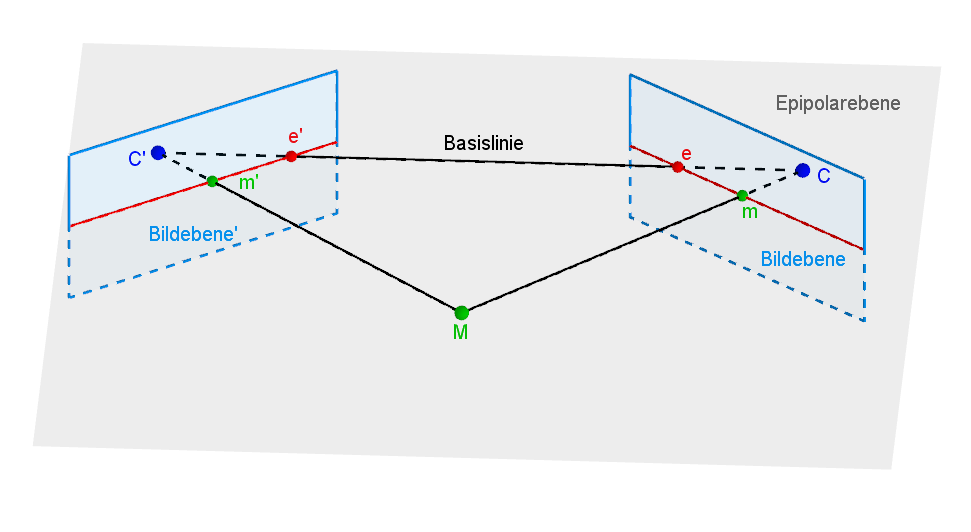
\includegraphics[width=.8\linewidth]{images/EpipolarGeoemtrieGrafik.png}
	\captionof{figure}{$C$ und $C'$ sind die Projektionszentren zweier Kameras. Beide Kameras besitzen jeweils eine Bildebene. Die Basislinien verbindet die Projektionszentren der Kameras. Der Punkt an welchem die Basislinie die Bildebenen schneidet, wird als Epipol bezeichnet. Durch den Epipol verlaufen alle Epipolarlinien des Bildes. $M$ ist der Objektpunkt im 3D-Raum und $m_1$ und $m_2$ sind die jeweiligen Abbildungen dieses Punktes auf den Bildebenen. Die Verbindungsvektoren zwischen $C, C'$ und $M$ bilden die sogenannte Epipolarebene\cite{Elements,HZ,ZZGXr}.}  
	\label{fig:Epipolargeometry}
\end{minipage}\\ \\

\begin{minipage}{\linewidth}
	\centering
	\includegraphics[width=1.\linewidth]{images/EpipolarLinien.png}
	\captionof{figure}{Die Objektpunkte $M_1, M_2$ und $M_3$ werden in $I'$ als $m'_1, m'_2$ und $m'_3$ abgebildet, während sie in $I$ immer den selben Bildpunkt $m_1$ ergeben.}  
	\label{fig:Epipolarconstraint}
\end{minipage}\\ \\

%Abbildung \ref{fig:Epipolarconstraint} veranschaulicht die soeben genannte Beziehung eines Bildpunktes zu seiner korrespondierenden Epipolarlinie noch mal grafisch. 

%Ist also nur Bildpunkt $m_\tau$ bekannt, so können alle Punkte auf dessen korrespondierender Epipolarlinie $l'$ mögliche korrespondierende Punkte zu $m_\tau$ sein. Der \textit{Epipolar-Contraint} kann durch $3 \times 3$-Matrizen ausgedrückt werden. Bei diesen Matrizen handelt es sich entweder um die Fundamentalmatrix $F$ oder die essentielle Matrix $E$\cite{HZ,ZZGXr,Elements,CamerModels.,Zhang2014}. Deren Herleitung und Beziehung, zu den korrespondierenden Bildpunkten, im weiteren Verlauf noch aufgezeigt wird. Der \textit{Epipolar-Contraint} gilt dann als erfüllt, wenn gilt, dass:
%
%
%
%\begin{gather}
%	m'^T_{\tau'} \cdot F \cdot m_\tau = 0\\
%	\bar{m}'^T_{\tau'} \cdot E \cdot \bar{m}_{\tau} = 0
%\end{gather}

%ergeben.


%
%
%
%Die essentielle Matrix und die Fundamentalmatrix unterscheiden sich darin, ob die intrinsischen Kameraparameter bekannt sind oder nicht. Die Fundamentalmatrix kommt dann zum Einsatz, wenn nur die Bildpunkte $m_\tau$ und $m'_{\tau'}$ bekannt sind, die Kameramatrizen $K$ und $K'$ und die Translationsmatrizen $R$ und $R'$ jedoch unbekannt sind. Man spricht hier von einem unkalibrierten Fall\cite{HZ,ZZGXr,Ferid}. Sind die intrinsischen Kameraparameter bekannt, so wird die Fundamentalmatrix $F$ zur essentiellen Matrix und man spricht von einem kalibrierten Fall$E$\cite{HZ,Elements}. Das Wissen über die Aussagen dieser \textit{Constraints} ist vor allem dann von Nutzen, wenn es darum geht aus einer Stereoskopischen Aufnahme anhand von korrespondierenden Bildpunkten die 3D-Szene zu rekonstruieren. Die korrespondierenden Punkte müssen zu Beginn der Stereobildanlayse erst einmal auf den Bilder ausfindig gemacht werden. Hierfür gibt es unterschiedliche Algorithmen, die in der \nameref{sec:einleitung} bereits erwähnt wurden. Wird einer dieser Algorithmen auf die Bilder angewandt, kann mit Hilfe des \textit{Epipolar-Constraints} deren Exaktheit der zueinander korrespondierenden Punkte überprüft werden\cite{Elements,ZZGXr,HZ}. 

\section{Bestimmung von Homographie und Fundamentalmatrix aus Punktekorrespondenzen}

(sollte vllt zwischen rein)
Hier sagen wo man die Punkte herbekommt

Im folgenden soll nun gezeigt werden, wie Homographien und Fundamentalmatrizen aus Punktekorrespondenzen gewonnen werden können. Für essentielle Matrizen gilt das selbe Verfahren wie für die Fundamentalmatrizen nur sind hier die Punktekorrespondenzen in normierten Koordinaten gegeben. Es wird davon ausgegangen, das die Transformationsmatrizen $R$ und $R'$ sowie die Kameramatrizen $K$ und $K'$ nicht bekannt sind. Des Weiteren gehen wir davon aus, dass zuvor mindestens acht korrespondierende Punkte aus den jeweiligen  Bildpaaren detektiert wurden. \\


Um eine Homographiematrix mit 
$H=
\begin{bmatrix}
h_{11}&h_{12}&h_{13}\\
h_{21}&h_{22}&h_{23}\\
h_{31}&h_{32}&h_{33}
\end{bmatrix}
$ zu erhalten werden die Punkte beider Kameras in eine Koeffizientenmatrix $A$ eingetragen, welche sich nach dem folgenden Schema aufstellen lässt. 

\begin{gather}
	H\cdot m_\tau = m'_{\tau}\\
	\begin{bmatrix}
		h_{11}&h_{12}&h_{13}\\
		h_{21}&h_{22}&h_{23}\\
		h_{31}&h_{32}&h_{33}
	\end{bmatrix}
	\cdot
	\begin{bmatrix}
		\\m_\tau\\\\
	\end{bmatrix}
	=
	\begin{bmatrix}
		\\m'_{\tau'}\\\\
	\end{bmatrix}\\
	\begin{bmatrix}
		h_{11}&h_{12}&h_{13}\\
		h_{21}&h_{22}&h_{23}\\
		h_{31}&h_{32}&h_{33}
	\end{bmatrix}
	\cdot
	\begin{bmatrix}
		x\\y\\z
	\end{bmatrix}
	=
	\begin{bmatrix}
		x'\\y'\\z'
	\end{bmatrix}
\end{gather}

Aus Gleichung 3.16 lässt sich das folgende Gleichungssystem aufstellen.  

\begin{gather}
	h_{11}x+h_{12}y+h_{13}z= \lambda x'\\
	h_{21}x+h_{22}y+h_{23}z= \lambda y'\\
	h_{31}x+h_{32}y+h_{33}z= \lambda z'
\end{gather}

Da mit zweidimensionalen homogenen Bildkoordinaten gearbeitet wird und somit $z$ und $z'$ = 1 sind, ergibt sich für die letzte Zeile $h_{31}x+h_{32}y+h_{33}z= \lambda$. Setzt man das anstelle von $\lambda$ ein, so ergeben sich die folgenden Gleichungen:

%Dieser Ausdruck kann in den ersten beiden Gleichungen für $\lambda$ eingesetzt werden. Pro Punktepaar $m_\tau$ und $m'_{\tau'}$ ergeben sich somit zwei Gleichungen. 

\begin{gather}
	h_{11}x+h_{12}y+h_{13}z= (h_{31}x+h_{32}y+h_{33}z) \cdot x'\\
	h_{21}x+h_{22}y+h_{23}z= (h_{31}x+h_{32}y+h_{33}z) \cdot y'
\end{gather}

Für den Aufbau von $A$ werden beide Ausdrücke noch nach Null aufgelöst, so dass sich die Gleichungen 4.34 und 4.35 aus 4.32 und 4.33 ergeben. Pro korrespondierendem Punktepaar $m_\tau$ und $m'_{\tau'}$ ergeben sich somit zwei Gleichungen:

\begin{gather}
	h_{11}x+h_{12}y+h_{13}z -(h_{31}x+h_{32}y+h_{33}z) \cdot x'= 0 \\	h_{21}x+h_{22}y+h_{23}z-(h_{31}x+h_{32}y+h_{33}z) \cdot y'=0
\end{gather}
\begin{gather}
	\leadsto h_{11}x+h_{12}y+h_{13}z -h_{31}x\cdot x' - h_{32}y \cdot x'-h_{33}z\cdot x'= 0\\
	\leadsto h_{21}x+h_{22}y+h_{23}z-h_{31}x\cdot y -h_{32}y \cdot y -h_{33}z) \cdot y'=0
\end{gather}

Die entstandenen Gleichungen werden dann nach folgendem Schema in die Koeffizientmatrix $A$ eingetragen.\cite{Elements,HZ,Schwarz,Heipke}

\begin{gather}
	\begin{pmatrix}
		x_1&y_1&1&0&0&0&x_1 x'_1&y_1 x'_1 & 1\cdot x'_1\\
		0&0&0&x_1&y_1&1&x_1 y'_1&y_1 y'_1 & 1\cdot y'_1\\
		&&&&&.&&&\\	
		&&&&&.&&&\\	
		&&&&&.&&&\\	
		x_i&y_i&1&0&0&0&x_i x'_i&y_i x'_i & 1\cdot x'_i\\
		0&0&0&x_i&y_i&1&x_i y'_i&y_i y'_i & 1\cdot y'_i
	\end{pmatrix}
	\cdot
	\begin{pmatrix}
		h1\\h2\\.\\.\\.\\hi
	\end{pmatrix}
	=0
\end{gather}

Gesucht wird nun ein Vektor $\vec{x}$, für den gilt das $A \cdot x = 0$. Der gesuchte Vektor $\vec{x}$ entspricht dem Kern der Koeffizientenmatrix und ist ein Spaltenvektor mit insgesamt neun Einträgen, welche in die 3x3-Homographiematrix eingetragen werden können\cite{HZ,Schwarz}.\\


%Die Ermittlung der Fundamentalmatrix $F$ mit den korrespondierenden Bildpunkten der beiden Kamerabilder erfolgt mit Hilfe des sogenannten  \textit{8-Point-Algorithms}\cite{HZ}.  
Das Verfahren mit welchem sowohl $F$ als auch $E$ geschätzt werden können, ähnelt in seinem Ablauf dem der Homographiebestimmung. Das Verfahren wird hier allgemein als der \textit{eigth-Point-Algorithm} bezeichnet. Der \textit{8-Point-Algorithm} ist eine lineare Technik die angewandt wird, um die Fundamentalmatrix, sowie auch die essentielle Matrix, aus  $n \geq 8$ Punkten schätzen zu können \cite{Zhang2014,HZ}. Der Algorithmus benötigt $n \geq 8$ Punkte, um ein valides Ergebnis zu liefern \cite{HZ,Ferid}. Das Ergebnis und jedes seiner Vielfachen ist eine mögliche Lösung für $F$. Das auch jedes Vielfache eine gültige Lösung ist, kann aus der Herleitung der Epipolargeometrie geschlossen werden. \textcolor{red}{(sagen warum aber ich weiß nicht wie genau man das sagt ohne wieder auszuschweifen ....)}. Der Algorithmus wird am Beispiel ür die Bestimmung von $F$ veranschaulicht. Zunächst wird auch hier eine Koeffizientenmatrix aus den detektierten Punktekorrespondenzen gebildet. 


\begin{gather}
	{m'}_{\sigma'}^T \cdot F \cdot m_\sigma =0\\
	F=\begin{bmatrix}
		f_{11}&f_{122}&f_{13}\\
		f_{21}&f_{22}&f_{23}\\
		f_{31}&f_{32}&f_{33}
	\end{bmatrix}\\
	\begin{bmatrix}
		x'_n&y'_n&1
	\end{bmatrix} 
	\cdot
	\begin{bmatrix}
		f_{11}&f_{122}&f_{13}\\
		f_{21}&f_{22}&f_{23}\\
		f_{31}&f_{32}&f_{33}
	\end{bmatrix}
	\cdot
	\begin{bmatrix}
		x_n\\y_n\\1
	\end{bmatrix} =0\\
	f_{11}x_nx'_n+f_{12}y_nx'_n+f_{13}x'_n+f_{21}x_ny'_n+f_{22}y_ny'_n+f{23}y'_n+f_{31}x_n+f_{32}y_n+f_{33} =0\\
	(x_nx'_n,y_nx'_n,x'_n,x_ny'_n,y_ny'_n,y'_n,x_n,y_n,1)\cdot f =0\\
	\begin{bmatrix}
		x_1x'_1&y_1x'_1&x'_1&x_1y'_1&y_1y'_1&y'_1&x_1&y_1&1\\
		x_2x'_2&y_2x'_2&x'_2&x_2y'_2&y_2y'_2&y'_2&x_2&y_2&1\\
		.&.&.&.&.&.&.&.&.\\
		.&.&.&.&.&.&.&.&.\\
		.&.&.&.&.&.&.&.&.\\
		x_nx'_n&y_nx'_n&x'_n&x_ny'_n&y_ny'_n&y'_n&x_n&y_n&1
	\end{bmatrix}
	\cdot 
	\begin{pmatrix}
		f_{11}\\f_{12}\\f_{13}\\f_{21}\\f_{22}\\f_{23}\\f_{31}\\f_{32}\\f_{33}
	\end{pmatrix}
	= 0
\end{gather}\\

Gesucht wird wieder ein Vektor $\vec{f}$, für den gilt das $A \cdot f = 0$. Der gesuchte Vektor $\vec{f}$ entspricht auch hier dem Kern von A und ist ein Spaltenvektor mit insgesamt neun Einträgen, welche in die 3x3-Fundamentalmatrix eingetragen werden können\cite{HZ,ZZGXr}.\\


Bei der Homographie wie auch bei der Fundamentalmatrix, kann es dazukommen ,dass das Gleichungssystem, welches für die Kernbestimmung beider Koeffizientenmatrizen gelöst wird, zu einem überbestimmten System wird. Ein System gilt als überbestimmt, wenn es durch mehr Gleichungen als Unbekannte beschrieben wird. Für die Koeffizientenmatrix für $F$ und $H$ hätte, dass zur Folge, dass die Koeffizientenmatrix in ihrem Rang steigt. Die Bestimmung des Kerns würde in beiden Fällen kein eindeutiges Ergebnis mehr liefern\cite{HZ}.  \\


Für die Lösung überbestimmter Systeme wird durch ein \textit{least-square}- Verfahren, mit Hilfe der Singulärwertszerlegung einer Matrix $A$ eine Lösung für einen Vektor $\vec{x}$ beziehungsweise gesucht, so dass $\parallel A \cdot x \parallel$ minimal wird \cite{HZ,Scholz,Schwarz}. Die Singulärwertzerlegung von $A$ ist eine Faktorisierung der Matrix \ensuremath{A \in \mathbb{R}^{m \times n}} der Form \ensuremath{A = U \cdot S \cdot V^T} mit orthogonalen Matrizen \ensuremath{U \in \mathbb{R}^{m \times n}} und \ensuremath{V \in \mathbb{R}^{m \times n}} sowie mit einer Diagonalmatrix $S$. 

 


\begin{gather}
	S = \begin{pmatrix}
		s_1&&...&&0&0&&...&&0\\
		.&.&&&.&.&&&&.\\
		.&&.&&.&.&&&&.\\
		.&&&.&.&.&&&&.\\
		0&&...&&s_r&0&&...&&0\\	
		0&&...&&0&0&&...&&0\\
		.&&&&.&.&&&&.\\
		.&&&&.&.&&&&.\\	
		.&&&&.&.&&&&.\\	
		0&&...&&0&0&&...&&0\\	
	\end{pmatrix}
\end{gather}

Die  Diagonalmatrix $S$ beherbergt die Singulärwerte der Matrix. Für die Singulärwerte in $S$ soll für $s_1$ bis $s_r$ gelten, dass \ensuremath{s_1 \geq s_2 \geq ... \geq s_r \ge 0 }\cite{Scholz}.Dabei soll für die diagonalen Singulärwerte in $S$ mit $s_1$ bis $s_r$ gelten, dass \ensuremath{s_1 \geq s_2 \geq ... \geq s_r \ge 0 }\cite{Scholz}. Die Spalte von $V^T$, welche mit dem kleinsten Singulärwert von $S$ korrespondiert, ergibt den Vektor $\vec{x}$, für den \ensuremath{\parallel A \cdot x\parallel} minimal wird. \\
 
  
  
%Beispielrechnungen, in denen die Homographiematrix einmal für den Fall des rotierten Projektionszentrums und einmal mit der Drehung um einen Drehpunkt mit durchgerechnet wurde befindet sich im  \nameref{sec:appendix} unter \ref{sec:AppendixHomographieRotationPZ} und \ref{sec:AppendixHomographieRotationDP}.





